\documentclass[11pt,compress,t,notes=noshow, xcolor=table]{beamer}
\usepackage[]{graphicx}\usepackage[]{color}
% maxwidth is the original width if it is less than linewidth
% otherwise use linewidth (to make sure the graphics do not exceed the margin)
\makeatletter
\def\maxwidth{ %
  \ifdim\Gin@nat@width>\linewidth
    \linewidth
  \else
    \Gin@nat@width
  \fi
}
\makeatother

\newcommand{\citebutton}[2]{%
\beamergotobutton{\href{#2}{#1}}%
}

\newcommand{\blu}[1]{\textcolor{blue}{#1}}
\newcommand{\org}[1]{\textcolor{orange}{#1}}
\newcommand{\ques}{\textbf{\textcolor{red}{Question:  }}}
\newcommand{\questionssofar}{\begin{frame}\frametitle{Any questions?}\end{frame}}

\newcommand\warning{%
 \makebox[1.4em][c]{%
 \makebox[0pt][c]{\raisebox{.1em}{\scriptsize!}}%
 \makebox[0pt][c]{\color{red}\normalsize$\bigtriangleup$}}}%

\definecolor{fgcolor}{rgb}{0.345, 0.345, 0.345}
\newcommand{\hlnum}[1]{\textcolor[rgb]{0.686,0.059,0.569}{#1}}%
\newcommand{\hlstr}[1]{\textcolor[rgb]{0.192,0.494,0.8}{#1}}%
\newcommand{\hlcom}[1]{\textcolor[rgb]{0.678,0.584,0.686}{\textit{#1}}}%
\newcommand{\hlopt}[1]{\textcolor[rgb]{0,0,0}{#1}}%
\newcommand{\hlstd}[1]{\textcolor[rgb]{0.345,0.345,0.345}{#1}}%
\newcommand{\hlkwa}[1]{\textcolor[rgb]{0.161,0.373,0.58}{\textbf{#1}}}%
\newcommand{\hlkwb}[1]{\textcolor[rgb]{0.69,0.353,0.396}{#1}}%
\newcommand{\hlkwc}[1]{\textcolor[rgb]{0.333,0.667,0.333}{#1}}%
\newcommand{\hlkwd}[1]{\textcolor[rgb]{0.737,0.353,0.396}{\textbf{#1}}}%
\let\hlipl\hlkwb

\usepackage{framed}
\makeatletter
\newenvironment{kframe}{%
 \def\at@end@of@kframe{}%
 \ifinner\ifhmode%
  \def\at@end@of@kframe{\end{minipage}}%
  \begin{minipage}{\columnwidth}%
 \fi\fi%
 \def\FrameCommand##1{\hskip\@totalleftmargin \hskip-\fboxsep
 \colorbox{shadecolor}{##1}\hskip-\fboxsep
     % There is no \\@totalrightmargin, so:
     \hskip-\linewidth \hskip-\@totalleftmargin \hskip\columnwidth}%
 \MakeFramed {\advance\hsize-\width
   \@totalleftmargin\z@ \linewidth\hsize
   \@setminipage}}%
 {\par\unskip\endMakeFramed%
 \at@end@of@kframe}
\makeatother

\definecolor{shadecolor}{rgb}{.97, .97, .97}
\definecolor{messagecolor}{rgb}{0, 0, 0}
\definecolor{warningcolor}{rgb}{1, 0, 1}
\definecolor{errorcolor}{rgb}{1, 0, 0}
\newenvironment{knitrout}{}{} % an empty environment to be redefined in TeX

\usepackage{alltt}
\newcommand{\SweaveOpts}[1]{}  % do not interfere with LaTeX
\newcommand{\SweaveInput}[1]{} % because they are not real TeX commands
\newcommand{\Sexpr}[1]{}       % will only be parsed by R
\newcommand{\xmark}{\ding{55}}%


\usepackage[english]{babel}
\usepackage[utf8]{inputenc}

\usepackage{dsfont}
\usepackage{verbatim}
\usepackage{amsmath}
\usepackage{amsfonts}
\usepackage{amssymb}
\usepackage{bm}
\usepackage{csquotes}
\usepackage{multirow}
\usepackage{longtable}
\usepackage{booktabs}
\usepackage{enumerate}
\usepackage[absolute,overlay]{textpos}
\usepackage{psfrag}
\usepackage{algorithm}
\usepackage{algpseudocode}
\usepackage{eqnarray}
\usepackage{arydshln}
\usepackage{tabularx}
\usepackage{placeins}
\usepackage{tikz}
\usepackage{setspace}
\usepackage{colortbl}
\usepackage{mathtools}
\usepackage{wrapfig}
\usepackage{bm}
\usepackage{amsmath}
\usepackage{pifont}

\usetikzlibrary{shapes.multipart,shapes,arrows,automata,positioning,calc,chains,trees, shadows}
\tikzset{
  %Define standard arrow tip
  >=stealth',
  %Define style for boxes
  punkt/.style={
    rectangle,
    rounded corners,
    draw=black, very thick,
    text width=6.5em,
    minimum height=2em,
    text centered},
  % Define arrow style
  pil/.style={
    ->,
    thick,
    shorten <=2pt,
    shorten >=2pt,}
}

\tikzstyle{vec}=[draw, rectangle, fill = white, minimum width=5mm, minimum height=1cm, inner sep = 2pt]

\usepackage{subfig}

% Defines macros and environments
\usepackage{../../style/lmu-lecture}


\let\code=\texttt
\let\proglang=\textsf

\setkeys{Gin}{width=0.9\textwidth}

\setbeamertemplate{frametitle}{\expandafter\uppercase\expandafter\insertframetitle}

\usepackage{bbm}
% basic latex stuff
\newcommand{\pkg}[1]{{\fontseries{b}\selectfont #1}} %fontstyle for R packages
\newcommand{\lz}{\vspace{0.5cm}} %vertical space
\newcommand{\dlz}{\vspace{1cm}} %double vertical space
\newcommand{\oneliner}[1] % Oneliner for important statements
{\begin{block}{}\begin{center}\begin{Large}#1\end{Large}\end{center}\end{block}}


%new environments
\newenvironment{vbframe}  %frame with breaks and verbatim
{
 \begin{frame}[containsverbatim,allowframebreaks]
}
{
\end{frame}
}

\newenvironment{vframe}  %frame with verbatim without breaks (to avoid numbering one slided frames)
{
 \begin{frame}[containsverbatim]
}
{
\end{frame}
}

\newenvironment{blocki}[1]   % itemize block
{
 \begin{block}{#1}\begin{itemize}
}
{
\end{itemize}\end{block}
}

\newenvironment{fragileframe}[2]{  %fragile frame with framebreaks
\begin{frame}[allowframebreaks, fragile, environment = fragileframe]
\frametitle{#1}
#2}
{\end{frame}}


\newcommand{\myframe}[2]{  %short for frame with framebreaks
\begin{frame}[allowframebreaks]
\frametitle{#1}
#2
\end{frame}}

\newcommand{\remark}[1]{
  \textbf{Remark:} #1
}


\newenvironment{deleteframe}
{
\begingroup
\usebackgroundtemplate{
\includegraphics[width=\paperwidth,height=\paperheight]{../style/color/red.png}}
 \begin{frame}
}
{
\end{frame}
\endgroup
}
\newenvironment{simplifyframe}
{
\begingroup
\usebackgroundtemplate{
\includegraphics[width=\paperwidth,height=\paperheight]{../style/color/yellow.png}}
 \begin{frame}
}
{
\end{frame}
\endgroup
}\newenvironment{draftframe}
{
\begingroup
\usebackgroundtemplate{
\includegraphics[width=\paperwidth,height=\paperheight]{../style/color/green.jpg}}
 \begin{frame}
}
{
\end{frame}
\endgroup
}
% https://tex.stackexchange.com/a/261480: textcolor that works in mathmode
\makeatletter
\renewcommand*{\@textcolor}[3]{%
  \protect\leavevmode
  \begingroup
    \color#1{#2}#3%
  \endgroup
}
\makeatother





\input{../../latex-math/basic-math.tex}
\input{../../latex-math/basic-ml.tex}

\usepackage{animate}

\newcommand{\learninggoals}{
\item Get to know speculative decoding
\item Learn about Minimum Bayes Risk (MBR) Decoding
}
\definecolor{texblue}{rgb}{0, 0, 1}
\def\myblue#1{\textcolor{texblue}{#1}}

\title{Decoding Strategies}
% \author{}
\institute{\href{https://slds-lmu.github.io/lecture_dl4nlp/}{slds-lmu.github.io/lecture\_dl4nlp}}
\date{}

\begin{document}
\lecturechapter{Current Research in Decoding}
\lecture{Deep Learning for NLP}

% ------------------------------------------------------------------------------

\begin{vbframe}{Speculative Decoding}
\citebutton{PyTorch}{https://pytorch.org/blog/hitchhikers-guide-speculative-decoding/}

\vfill

\begin{itemize}
    \item Models generate the output sequence token by token
    \item A lot of forward passes are required to generate a long sequence of tokens
    \item Is there a way to generate the same ouput but also save time?
    \item \textbf{Idea:} attach multiple speculative heads to the model to predict the $N+1^{st}$, $N+2^{nd}$, $N+3^{rd}$, etc. token
\end{itemize}

\vfill
    
\end{vbframe}

% ------------------------------------------------------------------------------

\begin{vbframe}{Speculative Decoding: Architecture}

\vfill

\begin{minipage}[c]{.4\textwidth}
    \vfill
    \begin{figure}
		\centering
		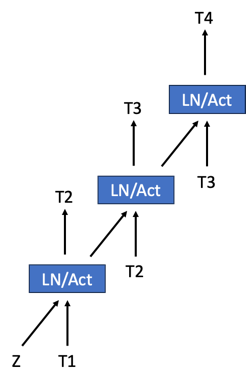
\includegraphics[]{chapters/chapter12/figure/spec_arc.png}
        \\ \citebutton{Speculator architecture}{https://pytorch.org/blog/hitchhikers-guide-speculative-decoding/#speculator-architecture}
	\end{figure}
    \vfill
\end{minipage}
\hfill
\begin{minipage}[c]{.49\textwidth}
    \hfill
    \begin{itemize}
        \item They base the architecture on the Medusa paper \citebutton{Cai et al., 2024}{https://arxiv.org/abs/2401.10774}
        \item Make heads hierarchical, where each head stage predicts a token and then feeds it into the next head stage
        \item $Z$ is the hidden state from the base model and $T1$, ..., $T4$ are the generated tokens
    \end{itemize}
\end{minipage}

    
\end{vbframe}
    
% ------------------------------------------------------------------------------

\begin{vbframe}{Speculative Decoding: Results}

\begin{figure}
    \centering
    \animategraphics[width=\textwidth, loop, autoplay]{8}%frame rate
    {chapters/chapter12/figure/gif/spec-}%path to figures
    {0}%start index
    {48}%end index
    \caption{Speed comparision between vanilla decoding (left) and speculative decoding (right) \citebutton{Gif}{https://pytorch.org/assets/images/hitchhikers-guide-speculative-decoding/fig1.gif}}
\end{figure}


    
\end{vbframe}

% ------------------------------------------------------------------------------

\begin{vbframe}{Speculative Decoding: Results}

\vfill

\begin{figure}
    \centering
    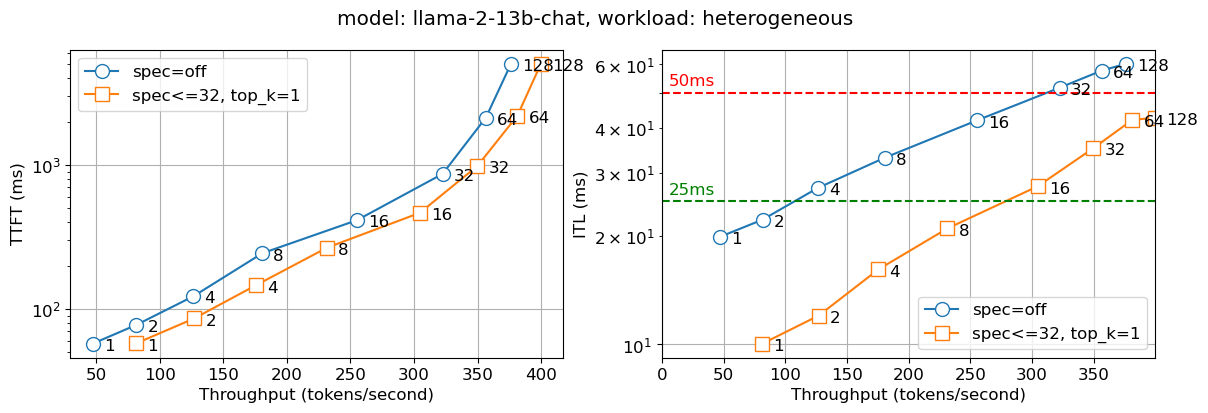
\includegraphics[]{chapters/chapter12/figure/spec_vs_no_spec.png}
    \caption{Time to first token (TTFT - left) and Inter-token latency (ITL - right) for Llama 13B with number of concurrent users indicated on the graph \citebutton{PyTorch blog}{https://pytorch.org/blog/hitchhikers-guide-speculative-decoding/#results}}
\end{figure}

\vfill

\end{vbframe}

% ------------------------------------------------------------------------------

\begin{vbframe}{Speculative Decoding: Training}

\begin{figure}
    \centering
    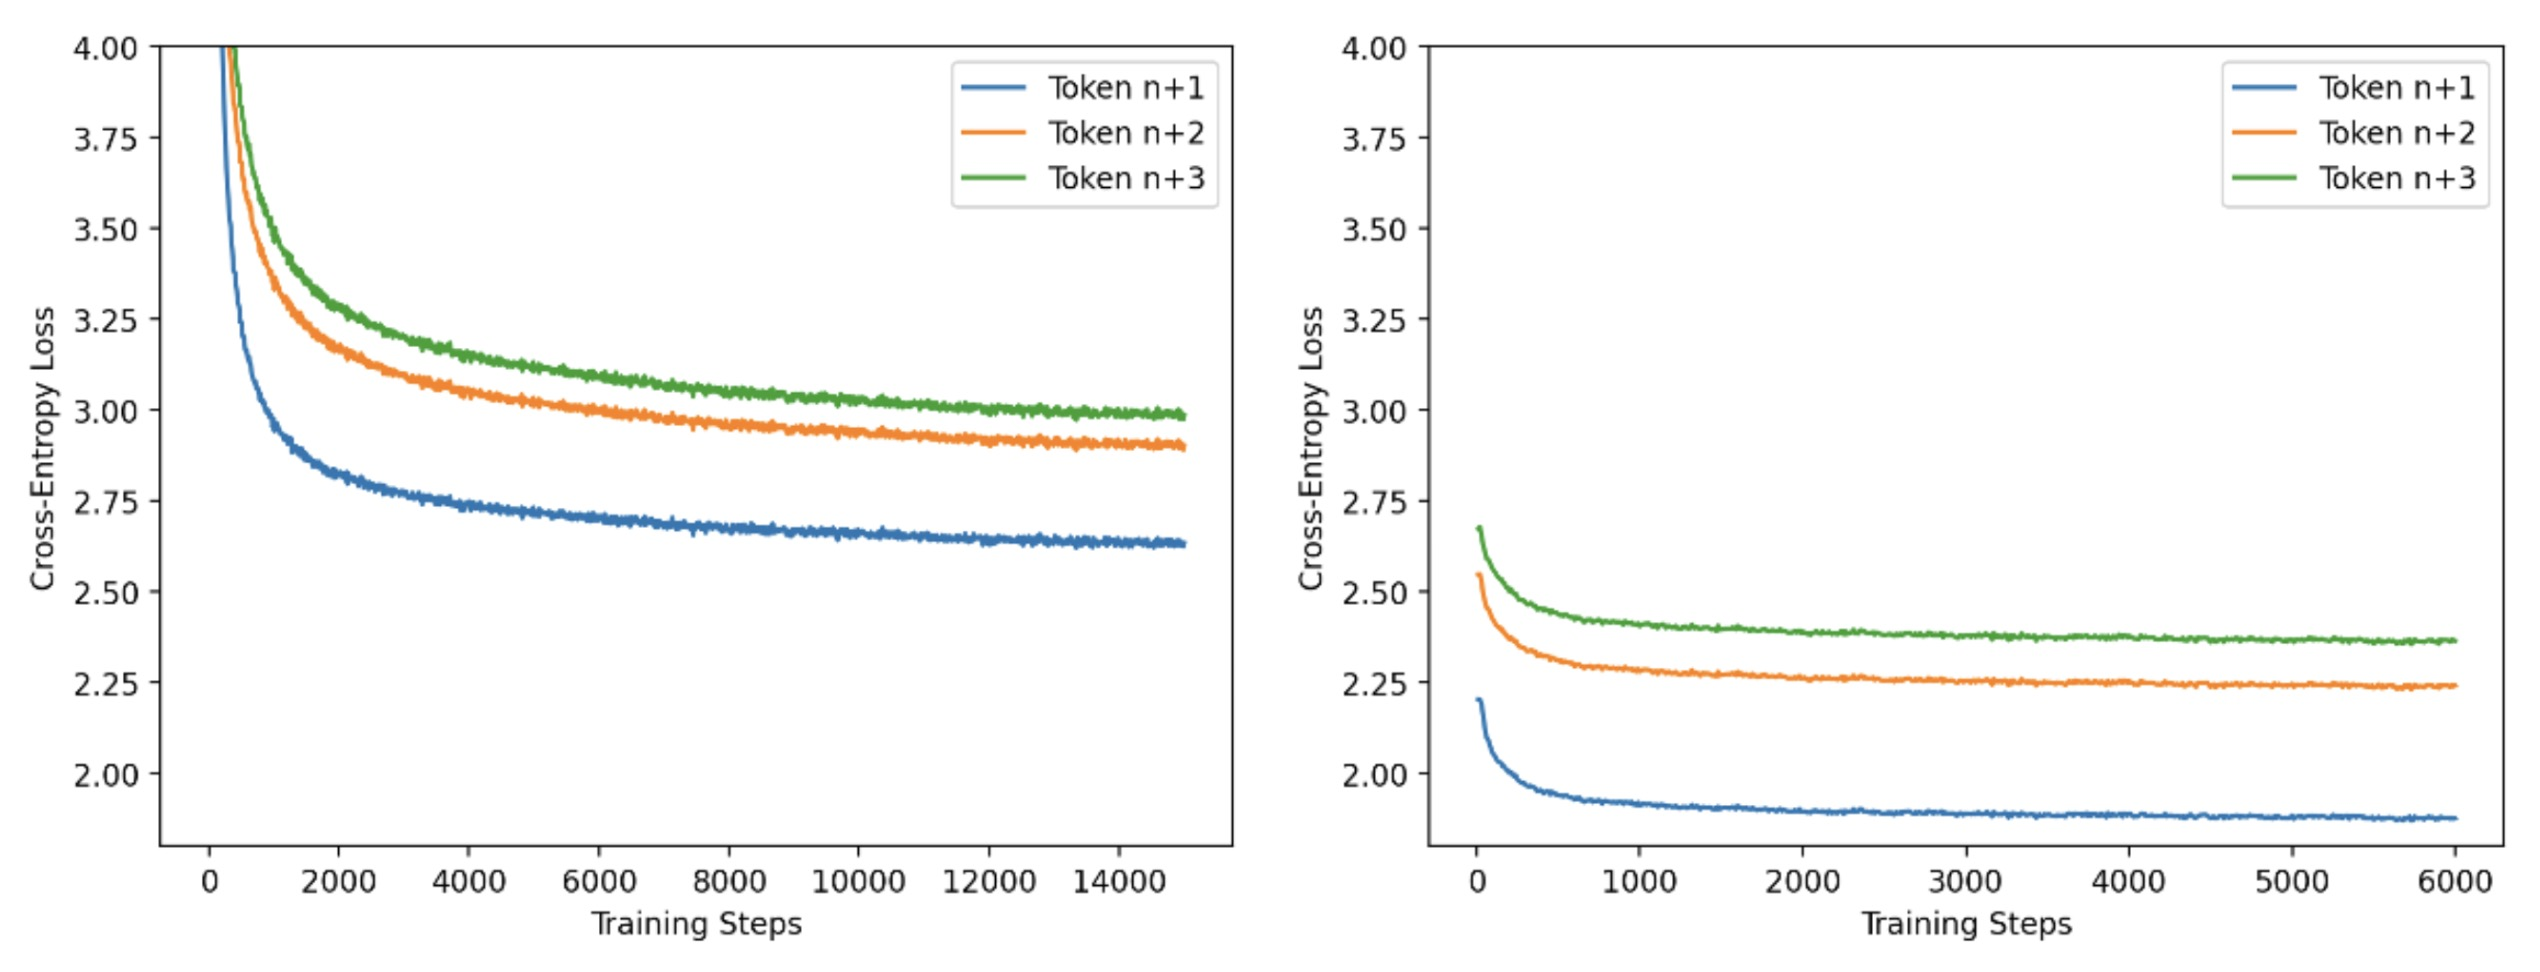
\includegraphics[]{chapters/chapter12/figure/spec_training.jpg}
    \caption{Per-head training loss curves for Llama2-13B speculator training, phase 1 and 2 \citebutton{PyTorch blog}{https://pytorch.org/blog/hitchhikers-guide-speculative-decoding/#results}}
\end{figure}

\begin{itemize}
    \item They use a two phase approach to training a speculator to be more efficient
    \item \textbf{Phase 1:} Train on small batches with long sequences (4k tokens) with standard causal LM approach
    \item \textbf{Phase 2:} Use large batches with short sequence lengths (256 tokens) generated from the base model 
    \item Tune the heads to match the output of the base model
\end{itemize}
    
\end{vbframe}

% ------------------------------------------------------------------------------

\begin{vbframe}{Minimum Bayes Risk (MBR) decoding}

\citebutton{GitHub, suzyahyah}{https://suzyahyah.github.io/bayesian\%20inference/machine\%20translation/2022/02/15/mbr-decoding.html}

\vfill

\begin{itemize}
    \item MBR is based on bayesian decision theory, where one would pick an action based on minimizing the \textit{Bayes Risk}:
    $$\alpha^* = \text{argmin}_{\alpha \in \mathcal{A}} \mathbb{E}_{\theta \sim p(\theta)}[\mathcal{L(\theta, \alpha)]}$$
    \item MBR Decoding involves choosing the bayes optimal action, where the action is a sequence
    \item Given a source input $x$ (i.e. source language in machine translation), the space of possible hypothesis $h \in \mathcal{H}(x)$, a probability distribution over decoded sequences $p(y|x)$, and a loss function $\mathcal{L}(y,h)$, the MBR decode is given by:
    $$h^* = \text{argmin}_{h \in \mathcal{H}(x)}\mathbb{E}_{p(y|x)}[\mathcal{L}(y,h))]$$
\end{itemize}

\vfill

\end{vbframe}

% ------------------------------------------------------------------------------

\begin{vbframe}{Minimum Bayes Risk (MBR) decoding}

\citebutton{GitHub, suzyahyah}{https://suzyahyah.github.io/bayesian\%20inference/machine\%20translation/2022/02/15/mbr-decoding.html}

\vfill

\begin{itemize}
    \item In theory we would like to have a distribution over reference sequences, which would be our $p(y|x)$
    \item But at inference time that is not available and we use $p_{\text{model}}(y|x)$ instead, as well as to construct $\mathcal{H}(x)$
    \item In practice MBR decoding has the following design choices (since its theoretical hypothesis space is infinite):
    \begin{itemize}
        \item Construction of the hypothesis space $\mathcal{H}(x)$
        \item Construction of the monte-carlo set of samples $y \in \mathcal{Y}$ to approximate $\mathbb{E}_{p(y|x)}$
        \item The choice of loss function $\mathcal{L}$, like BLEU, precision, etc. 
        \item Choosing how to renormalise samples $y$ from $p(y|x)$ with a small number of samples, the sequences are unlikely to be repeated and the monte-carlo estimate would give them all uniform probability
    \end{itemize}
\end{itemize}

\vfill

\end{vbframe}

% ------------------------------------------------------------------------------

\endlecture
\end{document}